\documentclass[11pt,a4paper]{article}
\usepackage[margin=2.2cm,headheight=16pt]{geometry}
\usepackage{babel}
\babelprovide[main]{spanish}
\setlocalecaption{spanish}{contents}{Contenido}
\usepackage{microtype}
\usepackage{xcolor}
\usepackage{graphicx}
\usepackage{booktabs}
\usepackage{longtable}
\usepackage{tabularx}
\usepackage{array}
\usepackage{enumitem}
\usepackage{fancyhdr}
\usepackage{lastpage}
\usepackage{titlesec}
\usepackage{listings}
\usepackage{amsmath}
\usepackage{amssymb}
\usepackage{tikz}
\usetikzlibrary{arrows.meta,positioning,shapes.geometric}
\usepackage[most]{tcolorbox}
\usepackage{hyperref}

\definecolor{MemBlue}{HTML}{1F49C4}
\definecolor{MemDark}{HTML}{161A21}
\definecolor{MemGray}{HTML}{4B5563}
\definecolor{MemLight}{HTML}{E7ECFA}
\definecolor{MemGreen}{HTML}{0D7355}
\definecolor{MemOrange}{HTML}{A06B06}
\definecolor{MemRed}{HTML}{AE382C}

\hypersetup{colorlinks=true,linkcolor=MemBlue,urlcolor=MemBlue,citecolor=MemBlue,
  pdftitle={Manual técnico de MemLab 16 MiB},pdfauthor={Documentación técnica del proyecto MemLab}}
\pagestyle{fancy}
\fancyhf{}
\lhead{\sffamily\small MemLab 16 MiB}
\rhead{\sffamily\small Manual técnico}
\cfoot{\sffamily\small Página \thepage\ de \pageref{LastPage}}
\titleformat{\section}{\Large\bfseries\sffamily\color{MemBlue}}{\thesection}{0.7em}{}
\titleformat{\subsection}{\large\bfseries\sffamily\color{MemDark}}{\thesubsection}{0.7em}{}
\titleformat{\subsubsection}{\normalsize\bfseries\sffamily\color{MemGray}}{\thesubsubsection}{0.7em}{}
\setlist{nosep,leftmargin=*}
\setlength{\parindent}{0pt}
\setlength{\parskip}{5pt}
\renewcommand{\arraystretch}{1.18}

\lstdefinestyle{memlab}{
  basicstyle=\ttfamily\footnotesize,
  keywordstyle=\color{MemBlue}\bfseries,
  stringstyle=\color{MemGreen},
  commentstyle=\color{MemGray}\itshape,
  backgroundcolor=\color{MemLight!45},
  frame=single,rulecolor=\color{MemBlue!25},
  breaklines=true,showstringspaces=false,tabsize=2,
  columns=fullflexible,
  numbers=left,numberstyle=\tiny\color{MemGray},numbersep=7pt,
  captionpos=b,keepspaces=true
}
\lstset{style=memlab}
\lstdefinelanguage{JavaScript}{
  keywords={break,case,catch,const,continue,debugger,default,delete,do,else,
    export,extends,false,finally,for,function,if,import,in,instanceof,let,new,
    null,return,static,super,switch,this,throw,true,try,typeof,var,void,while,with},
  morecomment=[l]{//},morecomment=[s]{/*}{*/},
  morestring=[b]",morestring=[b]'
}

\newtcolorbox{resumen}{colback=MemLight!55,colframe=MemBlue!70!black,
  boxrule=0.7pt,arc=2mm,title=Resumen técnico,fonttitle=\bfseries\sffamily}
\newtcolorbox{nota}[1][]{colback=gray!4,colframe=gray!45,
  boxrule=0.5pt,arc=1.5mm,title={#1},fonttitle=\bfseries\sffamily}
\newcommand{\archivo}[1]{\texttt{#1}}
\newcommand{\funcion}[1]{\texttt{#1()}}

\begin{document}

\begin{titlepage}
  \centering
  \vspace*{2.0cm}
  {\sffamily\bfseries\fontsize{34}{39}\selectfont\color{MemBlue} MemLab 16 MiB\par}
  \vspace{0.5cm}
  {\sffamily\fontsize{23}{28}\selectfont Manual técnico\par}
  \vspace{0.8cm}
  {\Large Simulador interactivo de gestión de memoria principal\par}
  \vfill
  \begin{tabular}{rl}
    \textbf{Versión documentada:} & estado local auditado el 23 de septiembre de 2026\\
    \textbf{Commit base observado:} & \texttt{20cec7a}\\
    \textbf{Plataforma:} & HTML5, CSS y JavaScript estándar\\
    \textbf{Espacio simulado:} & 16 MiB (\(2^{24}\) bytes)\\
  \end{tabular}
  \vfill
  {\small Documento generado exclusivamente a partir de \archivo{README.md},
  \archivo{index.html}, \archivo{css/style.css} y \archivo{js/script.js}.\par}
\end{titlepage}

\tableofcontents
\newpage

\section{Propósito, alcance y trazabilidad}

\begin{resumen}
MemLab es una aplicación web educativa, estática y de una sola página que modela
la asignación contigua de memoria sobre 16 MiB. Implementa particiones estáticas
iguales, particiones estáticas de tamaños variables y particiones dinámicas;
permite comparar primer, mejor y peor ajuste, observar fragmentación y ejecutar
compactación. No contiene servidor, base de datos, autenticación ni persistencia.
\end{resumen}

Este manual explica la arquitectura, el modelo de datos, los algoritmos, las
funciones, el renderizado, la ejecución, las dependencias y las restricciones del
estado actual del proyecto. La revisión se hizo sobre la copia de trabajo visible,
incluidas sus modificaciones locales, sin alterar los cuatro archivos originales.

\subsection{Inventario auditado}

\begin{longtable}{p{0.23\textwidth}p{0.13\textwidth}p{0.53\textwidth}}
\toprule
\textbf{Archivo} & \textbf{Líneas} & \textbf{Responsabilidad}\\
\midrule
\endhead
\archivo{README.md} & 105 & Visión general, ejecución y explicación conceptual.\\
\archivo{index.html} & 224 & Estructura semántica, controles, paneles, tabla, mapa y carga de recursos.\\
\archivo{css/style.css} & 331 & Sistema visual, temas claro/oscuro, estados de bloques, tablas y adaptación responsiva.\\
\archivo{js/script.js} & 783 & Estado, algoritmos de memoria, métricas, renderizado, bitácora y eventos.\\
\bottomrule
\end{longtable}

El código ejecutable suma 1\,338 líneas entre HTML, CSS y JavaScript. El archivo
JavaScript declara 33 funciones con nombre, más una función auxiliar de selección
del DOM y diversas funciones anónimas usadas como callbacks.

\section{Arquitectura del sistema}

\subsection{Estilo arquitectónico}

La solución sigue una arquitectura cliente monolítica y dirigida por eventos,
encapsulada en una IIFE (\emph{Immediately Invoked Function Expression}). Puede
entenderse como una separación ligera entre modelo, controladores y vistas:

\begin{itemize}
  \item \textbf{Modelo en memoria:} \texttt{cfg}, \texttt{mem}, \texttt{progs},
  \texttt{bitacora} y contadores auxiliares.
  \item \textbf{Lógica de dominio:} construcción de memoria, selección de huecos,
  carga, liberación, fusión, compactación y cálculo de métricas.
  \item \textbf{Controladores:} escuchadores DOM que traducen clics y cambios de
  formulario en mutaciones del modelo.
  \item \textbf{Vista:} funciones \texttt{render*} que regeneran HTML a partir del
  estado actual.
\end{itemize}

No existe un framework, enrutador, API ni almacén externo. El navegador contiene
todo el ciclo de vida y un refresco de página reinicia el sistema.

\subsection{Flujo de control}

\begin{center}
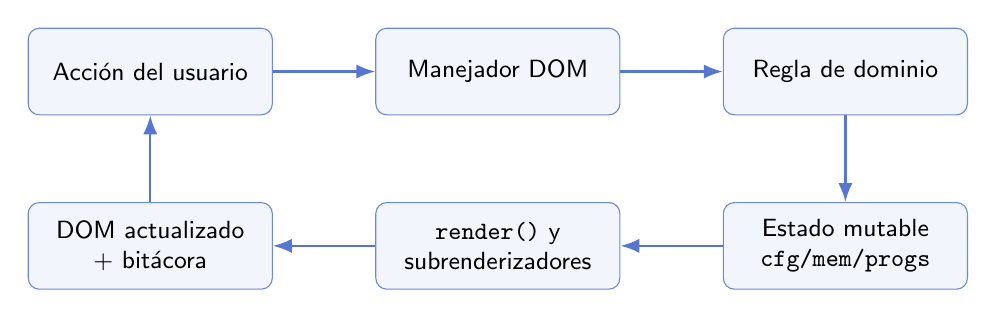
\begin{tikzpicture}[
  node distance=11mm and 13mm,
  box/.style={draw=MemBlue!65,rounded corners,fill=MemLight!55,
    minimum width=31mm,minimum height=11mm,align=center,font=\sffamily\small},
  arr/.style={-{Latex[length=2.4mm]},thick,color=MemBlue!75}
]
\node[box] (user) {Acción del usuario};
\node[box,right=of user] (event) {Manejador DOM};
\node[box,right=of event] (domain) {Regla de dominio};
\node[box,below=of domain] (state) {Estado mutable\\\texttt{cfg/mem/progs}};
\node[box,left=of state] (render) {\texttt{render()} y\\subrenderizadores};
\node[box,left=of render] (dom) {DOM actualizado\\+ bitácora};
\draw[arr] (user)--(event);
\draw[arr] (event)--(domain);
\draw[arr] (domain)--(state);
\draw[arr] (state)--(render);
\draw[arr] (render)--(dom);
\draw[arr] (dom)--(user);
\end{tikzpicture}
\end{center}

El patrón dominante es: evento \(\rightarrow\) mutación sincrónica
\(\rightarrow\) \funcion{render}. El renderizado completo es razonable porque el
estado es pequeño: decenas de bloques y procesos, no miles.

\subsection{Responsabilidades por capa}

\begin{description}
  \item[HTML.] Define la estructura estable y los puntos de montaje identificados
  por 33 IDs únicos. Incluye atributos ARIA en grupos, controles y bitácora.
  \item[CSS.] Usa variables personalizadas como tokens de diseño, sigue el esquema
  de color del sistema, reduce el mapa a una columna en pantallas de hasta 900 px y
  respeta la preferencia de movimiento reducido.
  \item[JavaScript.] Mantiene el estado privado dentro de la IIFE, procesa reglas
  de memoria, genera fragmentos HTML y conecta 14 grupos de interacciones.
\end{description}

\section{Modelo de dominio y estructuras de datos}

\subsection{Unidades y espacio de direcciones}

Las constantes principales son:
\[
  \texttt{KiB}=1024,\qquad \texttt{MiB}=1\,048\,576,\qquad
  \texttt{TOTAL}=16\times\texttt{MiB}=16\,777\,216\ \text{bytes}.
\]

Las direcciones válidas son \texttt{0x000000} a \texttt{0xFFFFFF}. Todos los
rangos mostrados son inclusivos, por lo que el extremo superior de un bloque es
\(base + size - 1\). La memoria de usuario es:
\[
  M_u=\texttt{TOTAL}-\texttt{cfg.so}.
\]

\subsection{Configuración \texttt{cfg}}

\begin{longtable}{p{0.19\textwidth}p{0.20\textwidth}p{0.48\textwidth}}
\toprule
\textbf{Campo} & \textbf{Valor inicial} & \textbf{Significado}\\
\midrule
\endhead
\texttt{metodo} & \texttt{"fija"} & Estrategia activa: fija, variable o dinámica.\\
\texttt{algo} & \texttt{"primero"} & Política de selección: primer, mejor o peor ajuste.\\
\texttt{so} & 2 MiB & Memoria residente reservada al sistema operativo.\\
\texttt{nFijas} & 7 & Cantidad de particiones iguales.\\
\texttt{variables} & 512, 1024, 1536, 2048, 3072, 6144 KiB & Tabla inicial de particiones distintas; suma 14 MiB.\\
\texttt{autoCompact} & \texttt{false} & Compacta al fallar por falta de continuidad si el total libre alcanza.\\
\bottomrule
\end{longtable}

\subsection{Bloque de memoria}

Cada elemento de \texttt{mem} es un objeto con \texttt{id}, \texttt{base},
\texttt{size}, \texttt{tipo}, \texttt{pid} y \texttt{fija}; las particiones
estáticas añaden \texttt{idx}. Los tipos posibles son:

\begin{itemize}
  \item \texttt{so}: bloque reservado al sistema operativo;
  \item \texttt{particion}: límite estático, libre u ocupado según \texttt{pid};
  \item \texttt{hueco}: espacio libre dinámico;
  \item \texttt{proceso}: bloque dinámico ocupado del tamaño exacto;
  \item \texttt{reservado}: sobrante no particionado e inutilizable.
\end{itemize}

El invariante esperado es que los bloques estén ordenados por dirección, no se
solapen y cubran todo el rango físico; los límites de las particiones estáticas no
se desplazan. En dinámica, \funcion{fusionar} mantiene la propiedad de que no
queden dos huecos contiguos separados después de una liberación.

\subsection{Proceso simulado}

Un proceso contiene \texttt{pid}, etiqueta \texttt{P\(n\)}, nombre, segmentos,
tamaño total en bytes, color, estado, base y bloque. Su tamaño es:
\[
  size=(codigo+datos+pila+heap)\times 1024.
\]

Los estados son \texttt{cola}, \texttt{cargado} y \texttt{rechazado}. Un rechazo
no elimina el trabajo: una liberación o compactación llama a
\funcion{limpiarRechazos} y lo devuelve a la cola.

\begin{longtable}{p{0.32\textwidth}rrrrr}
\toprule
\textbf{Programa} & \textbf{Código} & \textbf{Datos} & \textbf{Pila} & \textbf{Heap} & \textbf{Total KiB}\\
\midrule
\endhead
Editor de texto & 640 & 256 & 64 & 64 & 1\,024\\
Compilador C & 1\,280 & 512 & 128 & 128 & 2\,048\\
Navegador web & 1\,408 & 1\,024 & 256 & 1\,152 & 3\,840\\
Motor de base de datos & 768 & 1\,536 & 128 & 640 & 3\,072\\
Terminal & 192 & 96 & 32 & 128 & 448\\
Render 3D & 1\,024 & 2\,048 & 256 & 2\,816 & 6\,144\\
Servicio de red & 224 & 128 & 32 & 384 & 768\\
Hoja de cálculo & 512 & 768 & 64 & 192 & 1\,536\\
\bottomrule
\end{longtable}

El catálogo suma 18\,880 KiB, deliberadamente más que los 14 MiB de usuario de la
configuración predeterminada; esto permite observar admisiones y rechazos.

\section{Implementación explicada: código esencial}

Esta sección reproduce y explica el núcleo real de \archivo{js/script.js}. Se
incluye el código que determina el comportamiento del simulador; se omiten
principalmente cadenas de presentación, estilos y marcado repetitivo. La
numeración de cada listado es local al fragmento, mientras que el nombre de la
función permite encontrar su versión completa en el archivo fuente.

\subsection{Estado global, unidades y segmentos de un proceso}

\begin{lstlisting}[language=JavaScript,caption={Unidades, orden de segmentos y configuración inicial.}]
var KiB = 1024, MiB = 1048576, TOTAL = 16 * MiB;

var SEGS = [
  { k:"codigo", n:"Codigo",    c:"s-cod" },
  { k:"datos",  n:"Datos",     c:"s-dat" },
  { k:"pila",   n:"Pila",      c:"s-pil" },
  { k:"heap",   n:"Monticulo", c:"s-hea" }
];

var cfg = {
  metodo:"fija", algo:"primero", so:2 * MiB, nFijas:7,
  variables:[512, 1024, 1536, 2048, 3072, 6144],
  autoCompact:false
};

var mem = [], progs = [], bitacora = [];
var reloj = 0, sel = null, uid = 1, pid = 1;
\end{lstlisting}

\textbf{Lectura del código.} \texttt{TOTAL} fija un espacio de \(2^{24}\) bytes.
\texttt{SEGS} no guarda los valores de un proceso: define el orden canónico con el
que se suman y se dibujan código, datos, pila y montículo. \texttt{cfg} reúne las
decisiones que alteran la topología de memoria. \texttt{mem} contiene los bloques
físicos simulados y \texttt{progs} contiene los procesos; se mantienen separados y
se relacionan mediante \texttt{pid}.

\begin{lstlisting}[language=JavaScript,caption={Creación de un proceso y cálculo de su tamaño.}]
function nuevoPrograma(nombre, segs){
  var total = 0;
  for (var i=0; i<SEGS.length; i++){
    total += segs[SEGS[i].k];
  }
  return {
    pid: pid,
    etq: "P" + (pid++),
    nombre: nombre,
    segs: segs,
    size: total * KiB,
    color: COLORES[(pid - 2) % COLORES.length],
    estado: "cola",
    base: null,
    blk: null
  };
}
\end{lstlisting}

Los tamaños introducidos por la interfaz están en KiB. El bucle suma los cuatro
segmentos y luego multiplica una sola vez por 1\,024 para guardar \texttt{size} en
bytes. \texttt{base} y \texttt{blk} permanecen nulos hasta la admisión. Esta
separación evita mezclar unidades y permite calcular direcciones exactas.

\subsection{Cómo se particiona la memoria}

\begin{lstlisting}[language=JavaScript,caption={Tamaño de una partición fija igual.}]
function tamFija(){
  var usuario = TOTAL - cfg.so;
  return Math.floor(
    Math.floor(usuario / cfg.nFijas) / (4 * KiB)
  ) * (4 * KiB);
}
\end{lstlisting}

Primero se descuenta el S.O.; después se divide la memoria de usuario entre (N).
El segundo redondeo fuerza que la partición sea múltiplo de 4 KiB. Si la división
no es exacta, los bytes restantes no desaparecen: \funcion{construirMemoria} los
registra como zona reservada.

\begin{lstlisting}[language=JavaScript,caption={Construcción de los tres esquemas de memoria.}]
function construirMemoria(motivo){
  mem = [];
  mem.push({ id:uid++, base:0, size:cfg.so,
             tipo:"so", pid:null, fija:true });
  var base = cfg.so, i;

  if (cfg.metodo === "fija"){
    var ps = tamFija();
    for (i=0; i<cfg.nFijas; i++){
      mem.push({ id:uid++, base:base, size:ps,
                 tipo:"particion", idx:i+1, pid:null, fija:true });
      base += ps;
    }
  } else if (cfg.metodo === "variable"){
    for (i=0; i<cfg.variables.length; i++){
      var s = cfg.variables[i] * KiB;
      if (base + s > TOTAL) break;
      mem.push({ id:uid++, base:base, size:s,
                 tipo:"particion", idx:i+1, pid:null, fija:true });
      base += s;
    }
  } else {
    mem.push({ id:uid++, base:base, size:TOTAL-base,
               tipo:"hueco", pid:null, fija:false });
    base = TOTAL;
  }

  if (base < TOTAL){
    mem.push({ id:uid++, base:base, size:TOTAL-base,
               tipo:"reservado", pid:null, fija:true });
  }
  for (i=0; i<progs.length; i++){
    progs[i].estado = "cola";
    progs[i].base = null;
    progs[i].blk = null;
  }
  sel = null;
  if (motivo) addLog("config", motivo);
}
\end{lstlisting}

El puntero local \texttt{base} actúa como la siguiente dirección libre. En fija,
avanza siempre \texttt{ps}; en variable, avanza el tamaño indicado por la tabla;
en dinámica, toda la memoria de usuario empieza como un único hueco. El chequeo
\texttt{base + s > TOTAL} impide crear una partición fuera del rango físico. Una
reconfiguración invalida las direcciones anteriores, por eso todos los programas
regresan a cola.

\subsection{Selección: primer, mejor y peor ajuste}

\begin{lstlisting}[language=JavaScript,caption={Obtención y selección de bloques candidatos.}]
function libres(){
  return mem.filter(function(b){
    return b.pid === null &&
      (b.tipo === "particion" || b.tipo === "hueco");
  });
}

function elegir(cands){
  if (cfg.metodo === "fija") return cands[0];
  if (cfg.algo === "primero") return cands[0];
  var best = cands[0];
  for (var i=1; i<cands.length; i++){
    if (cfg.algo === "mejor"
        ? cands[i].size < best.size
        : cands[i].size > best.size){
      best = cands[i];
    }
  }
  return best;
}
\end{lstlisting}

\funcion{libres} excluye explícitamente el S.O. y la zona reservada. Antes de
llamar a \funcion{elegir}, \funcion{cargar} filtra además por capacidad. Por eso
\texttt{cands[0]} siempre es un bloque válido. Mejor ajuste conserva el menor;
peor ajuste conserva el mayor. En fija todos miden igual y se usa el primero.

\subsection{Carga y división de un hueco dinámico}

\begin{lstlisting}[language=JavaScript,caption={Búsqueda, compactación automática y admisión.}]
function cargar(id, silencioso){
  var p = prog(id);
  if (!p || p.estado === "cargado") return false;
  var l = libres();
  var cands = l.filter(function(b){ return b.size >= p.size; });

  if (!cands.length && cfg.metodo === "dinamica" &&
      cfg.autoCompact){
    var totalLibre = l.reduce(function(a,b){
      return a + b.size;
    }, 0);
    if (totalLibre >= p.size){
      compactar(true);
      l = libres();
      cands = l.filter(function(b){ return b.size >= p.size; });
    }
  }

  if (!cands.length){
    p.estado = "rechazado";
    return false;
  }

  var b = elegir(cands);
  if (b.fija){
    b.pid = p.pid;
  } else {
    if (b.size > p.size){
      var resto = {
        id:uid++, base:b.base + p.size,
        size:b.size - p.size,
        tipo:"hueco", pid:null, fija:false
      };
      b.size = p.size;
      mem.splice(mem.indexOf(b) + 1, 0, resto);
    }
    b.tipo = "proceso";
    b.pid = p.pid;
  }
  p.estado = "cargado";
  p.base = b.base;
  p.blk = b.id;
  return true;
}
\end{lstlisting}

La condición de admisión es \texttt{b.size >= p.size}. Si ningún hueco continuo
alcanza, la compactación automática solo se justifica cuando la suma libre sí es
suficiente. En una partición estática se asigna el PID sin cambiar el límite; la
diferencia queda como fragmentación interna. En dinámica se crea \texttt{resto}
con base \texttt{b.base + p.size}, se reduce el bloque original al tamaño exacto
del proceso y se inserta el hueco justo después. Así se conserva el orden de
direcciones y la fragmentación interna es cero.

\begin{nota}[Ejemplo numérico de división]
Si un hueco empieza en \texttt{0x200000}, mide 4 MiB y recibe un proceso de
1\,536 KiB, el proceso conserva la base \texttt{0x200000}. El nuevo hueco comienza
en \texttt{0x380000} y mide 2\,560 KiB. Los dos tamaños suman exactamente los
4 MiB originales; no se crean ni se pierden bytes.
\end{nota}

\subsection{Liberación y fusión de huecos contiguos}

\begin{lstlisting}[language=JavaScript,caption={Liberación de un proceso.}]
function liberar(id, silencioso){
  var p = prog(id);
  if (!p || p.estado !== "cargado") return;
  var b = null;
  for (var i=0; i<mem.length; i++){
    if (mem[i].pid === p.pid) b = mem[i];
  }
  if (!b) return;

  b.pid = null;
  var fusiones = 0;
  if (!b.fija){
    b.tipo = "hueco";
    fusiones = fusionar();
  }
  p.estado = "cola";
  p.base = null;
  p.blk = null;
  limpiarRechazos();
}
\end{lstlisting}

La liberación rompe el vínculo en ambos sentidos: el bloque pierde su PID y el
proceso pierde base e identificador de bloque. Una partición estática conserva su
tamaño. Un bloque dinámico recupera el tipo \texttt{hueco} y activa la fusión.

\begin{lstlisting}[language=JavaScript,caption={Coalescencia de huecos vecinos.}]
function fusionar(){
  var fusiones = 0;
  for (var i=0; i<mem.length-1; ){
    if (mem[i].tipo === "hueco" &&
        mem[i+1].tipo === "hueco"){
      mem[i].size += mem[i+1].size;
      mem.splice(i+1, 1);
      fusiones++;
    } else {
      i++;
    }
  }
  return fusiones;
}
\end{lstlisting}

El índice no avanza después de fusionar. Esto es intencional: si había tres
huecos seguidos, el bloque recién ampliado vuelve a compararse con el siguiente y
absorbe toda la cadena. La base del primero se conserva y el segundo se elimina.

\subsection{Compactación de memoria dinámica}

\begin{lstlisting}[language=JavaScript,caption={Reubicación de procesos y creación de un hueco final.}]
function compactar(auto){
  if (cfg.metodo !== "dinamica") return;
  var ocupados = mem.filter(function(b){
    return b.tipo === "proceso" && b.pid !== null;
  }).sort(function(a,b){ return a.base - b.base; });
  if (!ocupados.length) return;

  var base = cfg.so, movidos = 0;
  for (var i=0; i<ocupados.length; i++){
    if (ocupados[i].base !== base) movidos++;
    ocupados[i].base = base;
    var p = prog(ocupados[i].pid);
    if (p) p.base = base;
    base += ocupados[i].size;
  }

  var so = mem.filter(function(b){ return b.tipo === "so"; });
  mem = so.concat(ocupados);
  if (base < TOTAL){
    mem.push({ id:uid++, base:base, size:TOTAL-base,
               tipo:"hueco", pid:null, fija:false });
  }
  limpiarRechazos();
}
\end{lstlisting}

Ordenar por base conserva el orden relativo de los procesos. El acumulador
\texttt{base} comienza exactamente al final del S.O. y aumenta con cada tamaño,
por lo que no quedan huecos intermedios. Es indispensable actualizar tanto el
bloque como \texttt{p.base}; de otro modo, el mapa y el registro base mostrarían
direcciones distintas. Al final se reconstruye \texttt{mem}: S.O., procesos
contiguos y como máximo un hueco.

\subsection{Cálculo de uso y fragmentación}

\begin{lstlisting}[language=JavaScript,caption={Métricas derivadas del estado de memoria.}]
function metricas(){
  var usuario = TOTAL - cfg.so;
  var usado = 0, fragInt = 0, i, p;
  for (i=0; i<mem.length; i++){
    if (mem[i].pid !== null){
      p = prog(mem[i].pid);
      if (p){
        usado += p.size;
        fragInt += mem[i].size - p.size;
      }
    }
  }
  var l = libres();
  var libreTotal = l.reduce(function(a,b){
    return a + b.size;
  }, 0);
  var mayor = l.length ? Math.max.apply(null,
    l.map(function(b){ return b.size; })) : 0;
  var fragExt = cfg.metodo === "dinamica"
    ? libreTotal - mayor : libreTotal;
  return {
    usuario:usuario, usado:usado, fragInt:fragInt,
    libreTotal:libreTotal, mayor:mayor,
    huecos:l.length, fragExt:fragExt,
    util:usuario ? usado / usuario : 0
  };
}
\end{lstlisting}

\texttt{usado} suma tamaños reales de procesos, no tamaños de partición.
\texttt{fragInt} suma el sobrante dentro de cada bloque ocupado. En dinámica esa
diferencia siempre es cero gracias a la división exacta. \texttt{fragExt} resta
el mayor hueco al total libre: representa los bytes libres que no ayudan a cargar
un proceso limitado por el mayor tramo continuo.

\subsection{Cómo se distribuyen código, datos, pila y heap}

\begin{lstlisting}[language=JavaScript,caption={Cálculo de desplazamientos y rangos de cada segmento.}]
var off = 0;
for (i=0; i<SEGS.length; i++){
  var s = SEGS[i];
  var sz = p.segs[s.k] * KiB;
  var inicio = p.base + off;
  var fin = p.base + off + sz - 1;
  // La interfaz muestra: s.n, sz, off, inicio y fin.
  off += sz;
}
\end{lstlisting}

El simulador usa un modelo pedagógico contiguo: dentro del bloque del proceso se
ubican, en ese orden, código, datos, pila y heap. \texttt{off} comienza en cero;
el inicio de cada segmento es \texttt{p.base + off} y el final es inclusivo. Al
sumar \texttt{sz}, el siguiente segmento comienza exactamente un byte después.

\begin{nota}[Qué significa ``particionar la pila'' en este proyecto]
La pila no se administra como una partición física independiente ni crece durante
la ejecución. Es un segmento de tamaño fijo, expresado en KiB, dentro del bloque
contiguo asignado al proceso. El programa visualiza su rango y proporción, pero no
simula marcos de activación, punteros de pila, desbordamiento ni crecimiento hacia
direcciones menores. Esta precisión evita atribuir al simulador un comportamiento
que el código no implementa.
\end{nota}

\subsection{Actualización coherente de la interfaz}

\begin{lstlisting}[language=JavaScript,caption={Punto central de renderizado.}]
function render(){
  renderControles();
  renderKPIs();
  renderMapa();
  renderDetalle();
  renderProgs();
  renderLog();
}
\end{lstlisting}

Después de cada mutación importante, \funcion{render} vuelve a derivar controles,
indicadores, mapa, detalle, tabla y bitácora del mismo estado. No hay copias
independientes de los datos en la vista; esta decisión reduce inconsistencias en
una aplicación pequeña y sin framework.

\section{Algoritmos de gestión de memoria}

\subsection{Particiones estáticas de tamaño fijo}

La memoria de usuario se divide en \(N\) partes iguales, redondeadas hacia abajo a
múltiplos de 4 KiB:
\[
  P=\left\lfloor\frac{\left\lfloor M_u/N\right\rfloor}{4\,KiB}\right\rfloor
  \times 4\,KiB.
\]

Se crea una partición por cada índice; cualquier resto queda como zona
\texttt{reservado}. La carga usa la primera partición libre con capacidad
suficiente. El selector de ajuste se deshabilita porque todas las particiones
tienen el mismo tamaño. La fragmentación interna de un proceso es \(P-size\).

Con 2 MiB de S.O. y 7 particiones, \(P=2\) MiB y no queda sobrante. En el arranque
se cargan cuatro procesos que ocupan 5\,056 KiB útiles dentro de 8\,192 KiB
asignados; la fragmentación interna inicial es 3\,136 KiB.

\subsection{Particiones estáticas de tamaño variable}

\funcion{construirMemoria} recorre \texttt{cfg.variables} y crea una partición por
tamaño, siempre que su extremo no exceda \texttt{TOTAL}; al primer tamaño que no
cabe se interrumpe el bucle. Los tamaños añadidos por la interfaz se ordenan de
menor a mayor. Un proceso ocupa una partición completa y produce fragmentación
interna igual a \(\text{tamaño de partición}-size\).

Aquí sí se usa la política configurada. Las particiones libres no pueden unirse ni
compactarse porque sus límites son parte de la configuración estática.

\subsection{Particiones dinámicas}

El modelo comienza con un único hueco de \(M_u\). Al asignar un proceso:

\begin{enumerate}
  \item se filtran los huecos cuyo tamaño es al menos el del proceso;
  \item se selecciona uno según la política activa;
  \item si el hueco es mayor, se divide en un bloque de proceso exacto y un hueco
  residual situado inmediatamente después;
  \item el bloque elegido cambia de \texttt{hueco} a \texttt{proceso}.
\end{enumerate}

Por construcción no existe fragmentación interna. La liberación convierte el
bloque en hueco y fusiona vecinos libres contiguos. La fragmentación externa
aparece cuando el total libre se reparte entre varios huecos.

\subsection{Primer, mejor y peor ajuste}

Sea \(C\) la lista, en orden de dirección, de bloques libres que pueden contener
al proceso:

\begin{description}
  \item[Primer ajuste.] Devuelve \(C_0\). Costo de búsqueda completo: \(O(B)\),
  donde \(B\) es la cantidad de bloques; la selección posterior es \(O(1)\).
  \item[Mejor ajuste.] Recorre \(C\) y conserva el candidato de menor tamaño.
  Costo \(O(B)\); busca minimizar el resto inmediato.
  \item[Peor ajuste.] Recorre \(C\) y conserva el candidato de mayor tamaño.
  Costo \(O(B)\); busca dejar un resto grande potencialmente reutilizable.
\end{description}

No se mantienen índices, árboles ni listas segregadas; el objetivo es claridad
didáctica, no escalabilidad de un gestor real.

\subsection{Fusión de huecos}

\funcion{fusionar} recorre \texttt{mem} de izquierda a derecha. Si dos posiciones
consecutivas son huecos, suma sus tamaños y elimina la segunda sin avanzar el
índice; así puede absorber cadenas de tres o más huecos. Su costo es conceptualmente
\(O(B)\), aunque cada \texttt{splice} desplaza elementos y da un peor caso
\(O(B^2)\) en una implementación de arreglo. Para la escala de la simulación es
irrelevante.

\subsection{Compactación}

La compactación solo actúa en modo dinámico:

\begin{enumerate}
  \item obtiene los bloques de proceso y los ordena por base;
  \item coloca el primero justo después del S.O. y los demás de forma contigua;
  \item actualiza la base tanto del bloque como del proceso;
  \item reconstruye \texttt{mem} como S.O. + procesos + un hueco final, si sobra;
  \item devuelve procesos rechazados a cola y registra el número de movimientos.
\end{enumerate}

La complejidad es \(O(P\log P+B)\) por la ordenación de \(P\) procesos y los
filtrados sobre \(B\) bloques. La compactación automática se dispara únicamente
si no existe hueco suficiente pero la suma libre sí alcanza el tamaño solicitado.

\subsection{Métricas}

\funcion{metricas} calcula:

\begin{align*}
  usado &= \sum size(proceso\ cargado),\\
  fragInt &= \sum (size(bloque)-size(proceso)),\\
  libreTotal &= \sum size(bloque\ libre),\\
  mayor &= \max size(bloque\ libre),\\
  utilizacion &= usado/M_u.
\end{align*}

En modo dinámico, \(fragExt=libreTotal-mayor\), que expresa cuánto espacio libre
no pertenece al mayor tramo contiguo. En modos estáticos, el código presenta todo
el espacio de particiones libres como fragmentación externa, bajo la interpretación
didáctica de que esas particiones no pueden combinarse.

\section{Catálogo completo de funciones}

Las complejidades usan \(B\)=bloques, \(P\)=programas y \(S=4\)=segmentos.

\begin{longtable}{p{0.23\textwidth}p{0.51\textwidth}p{0.14\textwidth}}
\toprule
\textbf{Función} & \textbf{Contrato y efectos} & \textbf{Costo}\\
\midrule
\endhead
\funcion{hex} & Convierte un número a dirección hexadecimal mayúscula de seis dígitos. No muta estado. & \(O(1)\)\\
\funcion{miles} & Inserta separadores finos de millares en una representación decimal. & \(O(d)\)\\
\funcion{fmt} & Formatea bytes como KiB o MiB, con hasta dos decimales en MiB. & \(O(d)\)\\
\funcion{prog} & Busca por PID en \texttt{progs}; devuelve objeto o \texttt{null}. & \(O(P)\)\\
\funcion{esc} & Escapa \&, \textless, \textgreater{} y comillas para inserción HTML. & \(O(n)\)\\
\funcion{addLog} & Incrementa el reloj, antepone un evento y limita la bitácora a 80 filas. & \(O(P)\) por \texttt{unshift}\\
\funcion{nuevoPrograma} & Suma cuatro segmentos, asigna PID, etiqueta, color y estado inicial. Incrementa \texttt{pid}. & \(O(S)\)\\
\funcion{sembrarProgramas} & Reinicia PID y recrea los ocho programas base con copias de segmentos. & \(O(P)\)\\
\funcion{tamFija} & Calcula el tamaño igual redondeado a 4 KiB. & \(O(1)\)\\
\funcion{construirMemoria} & Reconstruye bloques según el método, devuelve procesos a cola, limpia selección y opcionalmente registra el motivo. & \(O(B+P)\)\\
\funcion{libres} & Filtra particiones o huecos sin PID. Excluye S.O. y reservado. & \(O(B)\)\\
\funcion{elegir} & Aplica primera, mínima o máxima capacidad sobre candidatos. & \(O(B)\)\\
\funcion{nombreBloque} & Produce una descripción humana según el tipo. & \(O(1)\)\\
\funcion{cargar} & Busca candidatos, compacta si corresponde, explica rechazos, divide huecos dinámicos y enlaza proceso/bloque. & \(O(B+P)\), más compactación\\
\funcion{liberar} & Localiza el bloque, limpia la asignación, fusiona huecos dinámicos y restablece rechazos. & \(O(B+P)\)\\
\funcion{fusionar} & Une huecos adyacentes y devuelve el número de fusiones. & hasta \(O(B^2)\)\\
\funcion{limpiarRechazos} & Convierte todos los estados rechazados en cola. & \(O(P)\)\\
\funcion{compactar} & Reubica procesos dinámicos hacia direcciones bajas y crea un hueco final. Registra resultado. & \(O(P\log P+B)\)\\
\funcion{metricas} & Agrega uso, fragmentación, huecos, reserva, procesos y utilización. & \(O(BP)\) por búsquedas PID\\
\texttt{\$(selector)} & Alias privado de \texttt{document.querySelector}. & según DOM\\
\funcion{render} & Orquesta controles, KPIs, mapa, detalle, programas y bitácora. & suma de subrenders\\
\funcion{renderControles} & Sincroniza pestañas, algoritmo, panel visible, textos, botones y chips. & \(O(V)\)\\
\funcion{renderKPIs} & Calcula métricas y monta cinco tarjetas. & \(O(BP)\)\\
\funcion{kpi} & Devuelve el HTML de una tarjeta y barra opcional. & \(O(1)\)\\
\funcion{renderMapa} & Genera un botón proporcional por bloque, fragmentación interna y clases por altura. & \(O(BP)\)\\
\funcion{renderDetalle} & Muestra rango, registro base/límite y tabla de segmentos del bloque seleccionado. & \(O(B+P+S)\)\\
\funcion{segbar} & Genera la barra proporcional de cuatro segmentos. & \(O(S)\)\\
\funcion{renderProgs} & Regenera filas, acciones, estados y suma del catálogo. & \(O(PS)\)\\
\funcion{renderLog} & Regenera hasta 80 eventos en orden inverso cronológico. & \(O(L)\)\\
\funcion{cargarTodos} & Intenta cargar los trabajos no cargados en orden y registra el total admitido. & \(O(P(B+P))\)\\
\funcion{liberarTodos} & Libera cada proceso cargado, registra cada efecto y el resumen. & \(O(P(B+P))\)\\
\texttt{escenario}\newline\texttt{Fragmentacion()} & Reinicia, carga en orden, libera posiciones alternas y sugiere un proceso pendiente. & \(O(P(B+P))\)\\
\funcion{reiniciar} & Restaura catálogo y memoria conservando la configuración activa. & \(O(B+P)\)\\
\funcion{arranque} & Inicializa el sistema, carga cuatro programas, selecciona el primer bloque y renderiza. & \(O(P(B+P))\)\\
\bottomrule
\end{longtable}

\section{Renderizado e interfaz}

\subsection{Mapa proporcional}

Cada bloque es un botón con \texttt{flex-grow} igual a su tamaño en bytes. Dentro
de un bloque ocupado estático, el contenido útil y la franja de fragmentación
interna reciben proporciones independientes. Después de insertar el DOM,
\funcion{renderMapa} mide la altura real y activa clases \texttt{tight} o
\texttt{micro} para reducir texto en bloques pequeños.

El mapa no dibuja píxeles por byte: normaliza mediante Flexbox dentro de una altura
CSS limitada por \texttt{clamp(430px, 70vh, 780px)}. Todos los valores numéricos y
rangos sí provienen del modelo exacto.

\subsection{Detalle de segmentos}

Cuando se selecciona un bloque ocupado, el desplazamiento empieza en cero y se
incrementa en el orden código, datos, pila y heap. Para cada segmento se muestra:
\[
  inicio=base+offset,\qquad fin=inicio+\text{tamaño}-1.
\]

El llamado ``registro límite'' mostrado por la interfaz es el tamaño del proceso en
hexadecimal, no la última dirección absoluta. Esto corresponde al uso didáctico de
un par base/límite.

\subsection{Bitácora}

Los eventos se anteponen con marcas \texttt{t001}, \texttt{t002}, etc. y se
clasifican como configuración, asignación, liberación, rechazo, compactación,
consulta o nota. Solo se conservan los 80 más recientes. La bitácora es estado
volátil y no se exporta.

\section{Eventos y ciclo de vida}

\begin{longtable}{p{0.28\textwidth}p{0.60\textwidth}}
\toprule
\textbf{Control} & \textbf{Efecto}\\
\midrule
\endhead
Pestaña de método & Cambia \texttt{cfg.metodo}, reconstruye toda la memoria y devuelve procesos a cola.\\
Selector de algoritmo & Cambia \texttt{cfg.algo}; registra la justificación.\\
Tamaño de S.O. & Convierte MiB a bytes y reconstruye memoria.\\
Número de particiones & Actualiza \texttt{nFijas} y reconstruye.\\
Chips variables & Eliminan por índice y reconstruyen.\\
Añadir partición & Valida mínimo y capacidad restante, ordena y reconstruye.\\
Compactar / automático & Compacta inmediatamente o activa el reintento automático.\\
Cargar / liberar & Invoca la regla sobre el PID de la fila y renderiza.\\
Clic en mapa & Alterna selección y registra una consulta.\\
Nuevo programa & Normaliza segmentos, valida contra memoria de usuario y agrega a cola.\\
Escenario & Recrea catálogo, carga lo posible y libera procesos alternos.\\
Reiniciar & Recrea estado operativo, pero conserva método y opciones actuales.\\
\bottomrule
\end{longtable}

\section{Ejecución, despliegue y compatibilidad}

\subsection{Ejecución directa}

No hay instalación ni compilación. Desde la raíz puede abrirse \archivo{index.html}
en un navegador moderno. También puede servirse localmente:

\begin{lstlisting}[language=bash]
cd /ruta/a/memlab
python3 -m http.server 8000
# abrir http://localhost:8000/
\end{lstlisting}

La ejecución sobre HTTP facilita depuración y evita restricciones particulares de
\texttt{file://}. Las fuentes de Google son la única dependencia de red; si no
están disponibles, la pila tipográfica usa fuentes del sistema y la funcionalidad
permanece intacta.

\subsection{Requisitos}

\begin{itemize}
  \item navegador con JavaScript habilitado, Flexbox, Grid, variables CSS y
  \texttt{color-mix}; se recomienda una versión moderna de Chrome, Edge, Firefox o Safari;
  \item resolución flexible; a 900 px o menos la cuadrícula pasa a una columna;
  \item no se requieren Node.js, paquetes npm, servidor de aplicación ni base de datos.
\end{itemize}

\subsection{Despliegue estático}

Puede publicarse tal cual en GitHub Pages, Netlify, Vercel estático, S3 u otro
servidor de archivos. Debe conservarse la relación de rutas
\archivo{index.html}, \archivo{css/style.css} y \archivo{js/script.js}. No existen
variables de entorno ni secretos.

\section{Validación realizada}

\begin{longtable}{p{0.32\textwidth}p{0.18\textwidth}p{0.38\textwidth}}
\toprule
\textbf{Prueba} & \textbf{Resultado} & \textbf{Evidencia}\\
\midrule
\endhead
Sintaxis JavaScript & Correcto & \texttt{node --check js/script.js} sin errores.\\
Servicio HTTP & Correcto & \texttt{index.html}, CSS y JS respondieron 200 con MIME apropiado.\\
Selectores DOM & Correcto & 33 IDs únicos; todos los selectores \texttt{\$("\#id")} existen.\\
Duplicados de ID & Correcto & No se detectaron IDs repetidos.\\
Revisión estática & Correcto & Se trazaron configuración, mutaciones, renderizado y eventos.\\
Prueba Playwright & No ejecutada & La dependencia Python Playwright no está instalada en el entorno.\\
\bottomrule
\end{longtable}

\section{Seguridad, accesibilidad y calidad}

\subsection{Controles existentes}

\funcion{esc} protege el nombre de usuario al representarlo en mapa, detalle y
tabla. Los controles principales cuentan con etiquetas ARIA, el registro usa
\texttt{aria-live="polite"}, hay foco visible y la animación solo se aplica cuando
el usuario no solicita reducción de movimiento.

\subsection{Hallazgos y limitaciones}

\begin{enumerate}
  \item \textbf{Inserción HTML en bitácora.} El nombre de un programa añadido se
  concatena sin escape al texto del evento y \funcion{renderLog} lo inserta con
  \texttt{innerHTML}. En un contexto compartido, un nombre con marcado podría
  convertirse en XSS DOM. Debe escaparse al registrar o al renderizar.
  \item \textbf{Sin persistencia.} Recargar la página elimina configuración,
  programas agregados, asignaciones y bitácora.
  \item \textbf{Tabla variable frente al S.O.} Cambiar el S.O. puede dejar una
  tabla configurada cuya suma exceda la memoria de usuario. El constructor ignora
  desde la primera partición que no cabe, mientras el texto de suma conserva toda
  la lista; conviene normalizarla o marcar explícitamente entradas omitidas.
  \item \textbf{Mensaje de rechazo fijo.} En ciertos casos con particiones libres
  demasiado pequeñas, el texto puede afirmar que ``todas están ocupadas'' cuando
  el problema real es capacidad individual insuficiente.
  \item \textbf{Compactación con memoria llena.} Si no queda espacio, el registro
  puede indicar ``1 hueco de 0 KiB'' aunque el arreglo no contenga hueco final.
  \item \textbf{Métrica didáctica.} En estáticas, llamar fragmentación externa a
  toda partición libre es una convención pedagógica; no es una definición universal.
  \item \textbf{Sin suite automatizada.} No hay pruebas unitarias, de integración
  ni end-to-end incluidas en el repositorio.
  \item \textbf{Compatibilidad CSS.} \texttt{color-mix} requiere navegadores
  recientes; no se define alternativa visual explícita para versiones antiguas.
\end{enumerate}

\section{Mantenimiento y extensión}

\subsection{Puntos de cambio habituales}

\begin{itemize}
  \item Para añadir un método, extender \texttt{cfg.metodo},
  \funcion{construirMemoria}, \funcion{cargar}, métricas, controles y textos.
  \item Para añadir una política, extender los botones, \texttt{ALGO\_POR\_QUE} y
  \funcion{elegir}.
  \item Para modificar segmentos, cambiar \texttt{SEGS}, el formulario, el modelo
  y el detalle; hoy varias partes asumen exactamente cuatro.
  \item Para persistencia, serializar configuración y programas; no conviene
  persistir IDs de bloques dinámicos porque se regeneran.
  \item Para pruebas unitarias, extraer la lógica de dominio de la IIFE a un módulo
  sin DOM y hacer explícitas sus entradas y salidas.
\end{itemize}

\subsection{Pruebas recomendadas}

\begin{enumerate}
  \item partición exacta, proceso un byte/KiB menor y proceso mayor;
  \item igualdad de candidatos en mejor y peor ajuste;
  \item liberación entre dos huecos y fusión triple;
  \item fallo por total insuficiente frente a fallo por falta de continuidad;
  \item compactación automática y manual, incluida memoria completamente llena;
  \item cambios 1/2/4 MiB de S.O. con todas las tablas variables;
  \item nombres con caracteres especiales y payloads HTML;
  \item navegación completa por teclado, lector de pantalla y ancho móvil.
\end{enumerate}

\section{Conclusión técnica}

MemLab implementa de forma compacta y legible un simulador didáctico de asignación
contigua. La estructura basada en estado privado, reglas sincrónicas y renderizado
centralizado es apropiada para su escala. Los algoritmos principales están
representados de manera fiel a su intención educativa: particiones estáticas,
división y fusión de huecos, tres ajustes y compactación. Las prioridades de una
evolución serían corregir el escape de la bitácora, aclarar casos límite de mensajes
y métricas, separar el dominio del DOM e incorporar pruebas automatizadas.

\end{document}
